\section{Work done to date}
\protect\label{section:workdonetodate}

The following outlines the work done to date.

\subsection{Database and Python tools}
\protect\label{section:databaseandtools}

In order to manage the large number of files, I set up a database using MySQL
and a Python library and tool set to access this conveniently. The
\textit{Numpy}, \textit{Scipy} and \textit{Matplotlib} libraries were used
extensively. For some GUI tools, I used \textit{PyQt}.

The library and tools were all written so as to be able to relocate the
databases and adjust various parameters without difficulty, and GUI tools were
created to manage those.

\subsubsection{Database}
\protect\label{seciion:database}

The database was set up to manage the following information:

\begin{enumerate}
  \item A record of each observation taken by the {\rem} telescope (including
  REMIR observations and observations not of the target).
  \item A record of each daily flat file taken.
  \item A record of each daily bias file taken.
  \item A record of each possible reference object for each of the {\rdwarf}
  targets, with possible aliases, magnitude and other relevant information
  including information on proper motions where appropriate.
  \item A record of each master flat file.
  \item A record of each master bias file.
  \item A cache of relevant FITS files.
  \item A record of the matching of objects to locations in the images.
  \item A record of the count of ADUs and uncertainties for the each matched
  object in each image.
\end{enumerate}

At the time of writing, this occupies 258GB.

Only relevant FITS files are saved in the cache; this is for the target
{\rdwarf} stars using the visible light filters. Other FITS files are not saved, but the software
toolset is set up to transparently fetch these if required.

\subsubsection{Python software}
\protect\label{section:softlib}

The software created offers the following functions:

\begin{enumerate}
  \item A library of routines for inclusion in Python scripts to manipulate the
  database and transparently download uncached FITS files, load list of
  objects close to a given set of coordinates subject to given criteria and
  applying proper motions where appropriate.
  \item Tools to perfect various functions, such as providing a comprehensive
  facility to list observations and objects subject to various criteria.
  \item Graphical GUI tools to adjust system parameters and handling of grey
  scales in images.
  \item A graphical display tool capable of extracting and displaying images,
  with options to save results to file such as in Fig. \ref{fig:initgexample},
  highlighting found results. If the mouse is held over an object in the
  display, basic data is displayed. If the right button is clicked whilst
  hovering over an object, a graphical tools is invoked to take various actions
  in relation to the object.
\end{enumerate}

\subsubsection{Graphical display}
\protect\label{section:graphicdisplay}

The contrast on many of the images is poor and some of the standard image
display software, such \textit{AperturePT} and \textit{AstroImageJ} struggled
with several images. I wrote to the author of \textit{AperturePT} attaching some
of the images and he commented on the poor contrast.

I wrote a GUI program using \textit{PyQt} which enabled me to choose the
combination of greyscales which best highlighted the images. If an image is
loaded by the program, the effects can be seen in real time on the image. An
example of the dialog boxes is shown in Fig. \ref{fig:geditorshot}.

\begin{figure}[!htbp]
\begin{center}
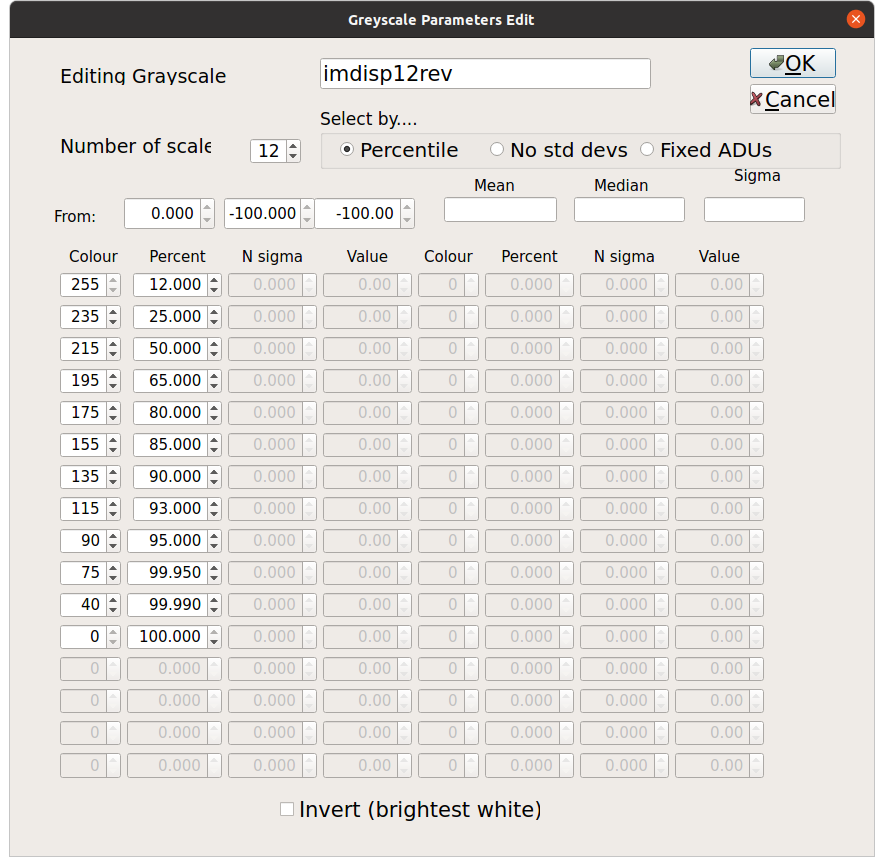
\includegraphics[scale=0.4]{images/geditorshot.png}
\end{center}   
\caption{This illustrates one of the dialogs from the graphical display editor
showing how the grey scales are tuned. Grey scales are assigned using
percentiles of the ADU values (default) by number of standard deviations or
absolute value. The values used are as shown in the figures. If an images is
loaded the other boxes are filled in to show the values from the current image
and updated, along with the figure displayed to show the effect on the image.
The results are saved in a configuration file for future use.}
\protect\label{fig:geditorshot}
\end{figure}

\subsection{Analysis of calibration files}
\protect\label{section:masterbiasflag}

In Fig. \ref{fig:mastmeanbias} is shown the mean value and standard deviation of
the master bias files up to March 2020.

\begin{figure}[!htbp]
\begin{center}
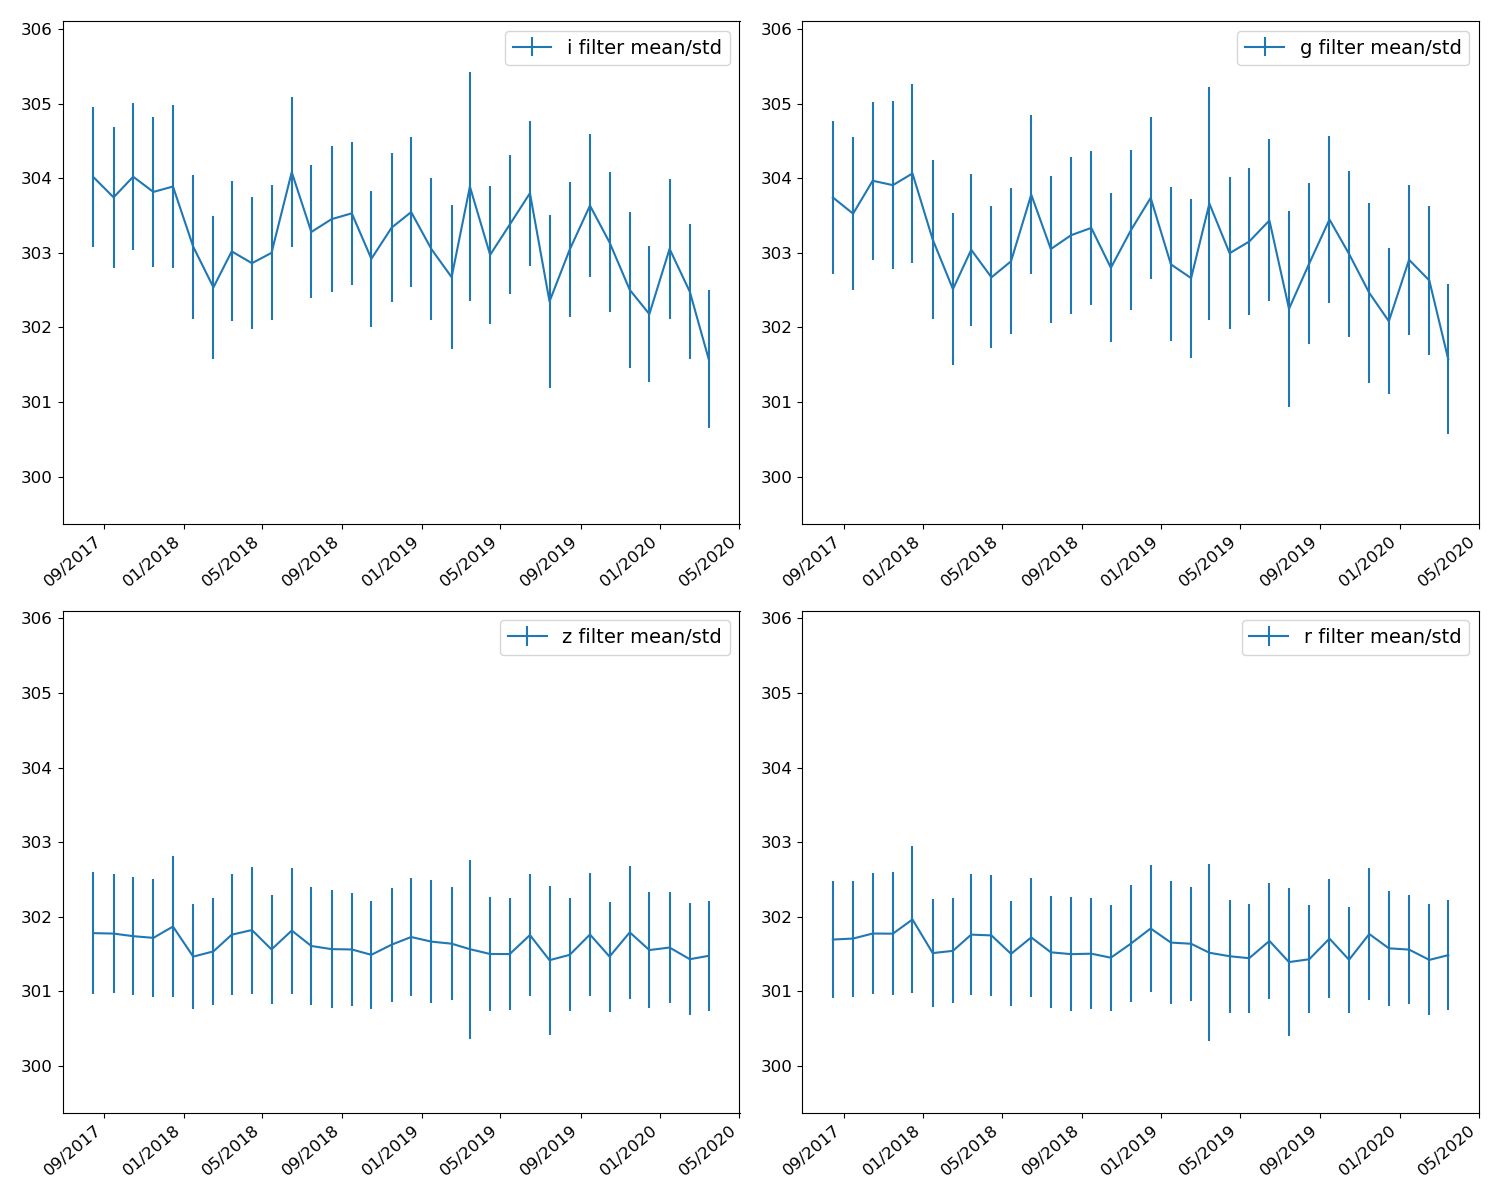
\includegraphics[scale=0.4]{images/mastmeanbias.png}
\end{center}   
\caption{This illustrates the mean and the standard deviation of the values in
the master bias files from July 2017, when {\rdwarf} targets were first
observed, until March 2020.}
\protect\label{fig:mastmeanbias}
\end{figure}
\clearpage

The master bias files are constructed from the daily bias files for the
corresponding month for each filter as follows:

\begin{enumerate}
  \item Tabulate the mean and standard deviation of each pixel count in each
  daily bias file for the month in question.
  \item Take the median mean (\textit{med\_e}) and the median standard deviation
  (\textit{sd\_e}) of those.
  \item Take the daily bias files whose mean in less than 3 times \textit{sd\_e}
  deviations away from \textit{med\_e}.
\end{enumerate}

Problems with this method appeared to be that the daily bias files are not
consistently compiled and the number can vary month to month. This accounts for
much of the variations in Fig. \ref{fig:mastmeanbias}. This is compounded by
some pixels getting ``stuck'' over a period and giving a high value for a string
of bias files. The effect of this is to give high values to pixels in the master
bias files which causes the pixels to become negative when the bias file is
subtracted from an image file.

Further problems are that the master bias file uses daily files up to a month
old and does not incorporate sufficient current behaviour. The overall standard
deviation is also a poor measure, in that many pixels are better than this in
terms of noise, others much worse.

I made the decision not to use the master bias files and construct a ``rolling''
master bias file centred on the date required. An uncertainty value is set for
each pixel based on all the daily bias files used.

There were similar and additional problems in the method of constructing the
master flat files. Examination of the IDL code used to construct the master flat
files revealed  that the master flat files were constructed using the daily flat files for the
relevant month, selected according to the criteria.

\begin{enumerate}
  \item The mean values of the pixel counts falls within the range 5,000 and
  50,000.
  \item The skewness of the distribution of the pixel counts is negative.
  \item The kurtosis of the distribution of the pixel counts is less than 7.
\end{enumerate}

All of these criteria are applied; a daily flat file is not selected if it does
not meet all these criteria. The justification for using the skewness and
kurtosis in this way is not clear.

Regrettably the calculation of the mean, skewness and kurtosis is not correct,
due to a programming error. Further, the history of the master flat file shows
all daily flat files considered for inclusion, not the ones actually selected.
\footnote{It did not seem a productive use of time to reproduce the programming error
and work out the actual but incorrect set of daily flat files which went to make
up the master flat files.}

Finally the pixel values are combined by taking the median value and then
normalised. This would appear to be a mistake as the daily flat files are
typically in groups of three as the light fades and thus only values from the
set of ``middle'' flat files would be selected. The files are normalised to the
median value not the mean, but this is not correct.

It was again decided to replace the master flat files with a ``rolling window''
of a fixed number of daily flat files centred on the date of the observation.
As with the replaced master bias files, standard deviations are constructed for
each individual pixel. An extensive study of the linearity was undertaken using
the daily flat files; it would  appear than the performance is linear up to
62,000 counts per pixel out of a possible 65,536. The master flat files were
selected using files with pixels between a range of 5,000 and 61,000 to be clear
of this linearity cut-off. None of the image files, other than ones contaminated
by cosmics and similar, had pixel values close to 60,000. With reasonable limitations on the flat files,
limiting the maximum standard deviations to 10,000 that the
majority are much less than this), files with positive skewness are reduced to
zero and those with kurtosis over 7 are negligible (under 0.01\%). References to
skewness and kurtosis did not seem relevant\footnote{Even if they were correctly calculated.} and hence for
construction of alternative master flat files, these were omitted.

The daily flat files are normalised first before being combined together to
construct the master flat file. These are then combined using a weighted
geometric mean, weighted to give the brighter files, with their higher SNR,
priority over the darkest files.

When the object ADU counts from {\rem} images are computed from the images, the
standard deviations for each individual pixel in the image are combined into an
overall standard deviation for the ADU count for the relevant object.

\subsection{Hotspots or defective pixels}
\protect\label{section:hotspots}

A study was undertaken of all the files, flat files, bias files and observation
files to determine whether any pixels in the CCD array could be counted as
``bad'' or unresponsive, had particularly high mean values or large standard
deviation. The literature varies somewhat on how bad pixels are defined or
determined.

Of recent papers, \citet{allers20} define bad pixels as ``dead'' pixels or pixels
with an uncertainty in the flat fields of over 10\%. In \citet{piskunov20} bad
columns in the CCD used are first identified and eliminated and then an
iterative procedure is adopted to effectively assign weights to each pixel. In
\citet{bongiovanni19} a procedure based on constructing two composite flat
fields from low and high counts and regarding as bad the pixels where the ratios
differ by more than 15\%. In \citet{belli18} a bad pixel mask is constructed by
selecting pixels in the flat fields with very low counts and those in the dark
frames with very high counts (but the criteria for ``low'' and ``high'' counts
in those files are not defined). In \citet{briesemeister18} pixels in the
constructed flat fields with values less than 0.5 or greater than 1.5 are
considered to be bad.

A comprehensive study of the quality of pixels is described in the
recently-published \citet{maslennikova20}. Pixels are described as
\textbf{Normal}, \textbf{Cold}. \textbf{Warm}. \textbf{Dead}, \textbf{Hot} and
\textbf{Inverse} according to the responses. The pixels on the ROSS2 telescope
CCD do not fit neatly into these brackets, apart from the \textbf{Normal} ones.

For the purposes of this study, the following definitions are used.

\begin{description}
\item[Normal] pixels are those which are clearly well-behaved with a linear
response within 10\% of saturation.
\item[Bad] pixels are closest to \textbf{Dead} pixels as defined in 
\citet{maslennikova20}. Included are those with consistent high levels of noise,
with the standard deviation on the bias level over 5 times the standard
deviation and those.
\item[Unreliable] pixels are ones which whilst otherwise normal, can randomly
give very high or low readings.
\end{description}

There are very few examples, in the order of 25 pixels spread over the used area
of the array, which qualify as \textbf{bad}, but the pixels which are
\textbf{unreliable} are of the order of about 11,000 over the array, spread over
the 4 areas used. Where detected, it is straightforward to interpolate over the
relevant pixels. There are a few places where there are strings of
adjacent unreliable pixels, but these almost entirely affect columns in the CCD,
the worst example can be found in the area used for the \gfilter, seemingly as
the CCD is read out by columns, so adjacent pixels on the same row have to be
used for interpolation.

\subsection{Finding and identifying objects}
\protect\label{section:findingidentify}

Most of the objects in the neighbourhood of the target {\rdwarf} objects were
identified using GAIA DR3. Where alternative shorter names than GAIA DR3 nnnnnnn
were found, this was used in preference. Bearing in mind the resolution of the
{\rem} telescope of around 0.6 arcsecond, objects closer together than this
distance were eliminated, as were objects with irregular profiles and one marked
as variable.

The magnitudes in various bands are all noted in the database records, but these
were mainly used as a guideline where there was ambiguity in distinguishing
close but not overlapping objects. It proved better to explicitly count the ADUs
after adjusting the aperture sizes.

There remains considerable work in finalising the optimal aperture sizes for
each objects, particularly with {\prox} and {\bstar}.

The best frames contain up to 200 possible reference stars for the best
examples, more for {\prox} and less for {\bstar}. Average frames contain up to
30 or so. Any less than 10 are rejected as too poor in contrast, but the total of rejected frames is less than
10\%.\footnote{This figure ia subject to amendment, currently the rejection is
binary, but there is provision for a ``quality'' marker enabling frames to be
partially used where appropriate.}

\subsection{Calibration of reference stars and ADU counts}
\protect\label{section:calibrationrefstars}

Not all the frames contain the same reference stars, or have the same
orientation, some are rotated by 90\degree or 180\degree relative to others. The
target object may be off-centre by varying amounts and in varying directions and
different reference objects appear in different frames, or are too close to the
edge in some cases, where vignetting or similar reduces the accuracy, to be
usable. Only quite a small handful of objects appear in all the frames.

After some experimentation with strategies for computing and calibration of the
objects, the most promising strategy emerged as being for each filter
(initially this was only done with the {\rfilter} images, being the least
problematic).

\begin{enumerate}
  \item Compute the ADU count and standard deviation for each object in each
  frame.
  \item Compute the mean ADU count and corresponding standard
  deviation for each object. Clearly strongly variable objects previously missed can be weeded out
  at this stage.
  \item For each observation, perform a linear regression fit of the calculated
  ADUs for each object other than the target in the frame to the mean ADUs.
  \item Apply the fit backwards, propagating the standard deviation, to the
  calculated ADUs for the target on the frame and compare with the mean ADUs for
  the target to give the variation from the mean of the target for that frame.
\end{enumerate}

This technique proved very successful, in most cases the correlation of the
linear regression was better than 95\%, and proved insensitive to what set of
reference stars were available on a particular frame.

The results for {\ross} are set out in the draft paper attached to this report.

\subsection{Set up of pipeline}
\protect\label{section:pipeline}

A daily routine was set up to interrogate the {\rem} results and load new data
into the database. The steps were:

\begin{enumerate}
  \item Load information about new observations into the database. This is just
  a simple record of information.
  \item Load FITS files corresponding to the ROSS2 observations of the target
  objects into the database cache.
  \item For loaded FITS files, add data about statistics such as maximum and
  minimum pixel values, mean and standard deviations into the database.
  \item For database rows corresponding to the targets, compute the barycentric
  dates and add to the database.
  \item Identify the target and other objects in the frames and add locations to
  the database. Mark frame as too poor to use if the target is not found, and
  less than a given number of reference objects, currently 10, are not found.
  \item Load FITS files corresponding to daily flat and bias files into the
  database.
  \item Load any new master bias and flat files (although these are no longer
  used).
\end{enumerate}

The calculation of ADUs for objects is currently done manually when ready, but
ultimately this will be added to the pipeline. Currently the daily job takes
about 40 minutes to run.
